\documentclass[conference,a4paper]{IEEEtran}
\usepackage{graphicx}
\usepackage{booktabs}
\usepackage{amsmath}
\usepackage{hyperref}
\usepackage{cite}
\usepackage{microtype}
\usepackage{enumitem}
\usepackage{float}
\setlist[itemize]{itemsep=1pt, topsep=2pt, parsep=0pt}

%% Float placement: allow more content per page before forcing a new page.
\renewcommand{\topfraction}{0.95}
\renewcommand{\bottomfraction}{0.9}
\renewcommand{\textfraction}{0.05}
\renewcommand{\floatpagefraction}{0.85}
\renewcommand{\dbltopfraction}{0.95}
\renewcommand{\dblfloatpagefraction}{0.85}
\setcounter{topnumber}{4}
\setcounter{bottomnumber}{4}
\setcounter{totalnumber}{6}
\setcounter{dbltopnumber}{4}

\hypersetup{colorlinks=true, linkcolor=black, citecolor=black, urlcolor=black}

\title{Cross-layer brokerage in area-crime-outcome police networks}

\author{\IEEEauthorblockN{ECMM447 CW2, UoE,
760012524}}

\begin{document}
\maketitle

\begin{abstract}
Recorded crime data is typically published as separate frequency tables,
hiding the relational structure that links areas, crime categories and
recorded outcomes within every individual record.
Six months of UK police-recorded crime for three forces are modelled as
a weighted multilayer network with crime type as the shared mediator
node between an area-crime layer and a crime-outcome layer.
A four-component composite brokerage score (area spread, outcome
connectivity, outcome entropy and weighted-distance betweenness)
ranks crime categories as cross-layer brokers.
Violence and sexual offences is the dominant broker in all three
forces; drugs is a consistent second-tier broker not visible from raw
event-count rankings.
A PageRank robustness check gives similar broker rankings to
betweenness (rank correlations 0.85 to 0.92) and a complementary
cosine-similarity community detection on outcome profiles supports a
broadly similar property-crime / violence-disorder community structure.
\end{abstract}

\section{Introduction}

Crime data is routinely published as separate frequency tables treating
three connected dimensions as independent counts.
Every crime record links an approximate area to a crime category and a category to a recorded outcome. Categories that connect many local areas to many recorded outcomes are not visible from simple marginal rankings alone.
Network analysis makes those connections the primary object of study
rather than a side-effect of aggregation.

Generic graph datasets used in earlier module coursework lack
the layered node-type structure needed to model
area-crime-outcome relationships.
I chose UK Police Open Data~\cite{ukpoliceopendata} because its
three-field record structure (approximate location, crime category,
recorded outcome) maps directly onto a multilayer bipartite
design~\cite{kivela2014multilayer}.
I excluded stop-and-search data because outcome availability differs
across forces.
I selected three England and Wales forces to allow regional
comparison under a consistent legal and recording
framework~\cite{tompson2015policeuk}.
Open police data supports spatial analysis but has known
accuracy, anonymisation and recording-completeness
limits~\cite{tompson2015policeuk}.
Prior work used bipartite projections to infer hidden offender
ties~\cite{isah2015bipartite}; this project instead models structural
associations between areas, categories and outcomes, not
person-level inference.

The research question is: \textit{which recorded crime categories act
as cross-layer brokers between Lower Layer Super Output Areas
(LSOAs) and recorded police
outcomes and how consistent are these brokerage roles across
Metropolitan Police Service, West Midlands Police and South Wales Police?}

\section{Data and Methods}

\subsection{Dataset and network construction}

Street-level crime CSV files for November~2025 to April~2026 were
downloaded from \texttt{data.police.uk} per force and reduced to
force, LSOA code, crime type and \texttt{Last outcome category}.
Records without an LSOA were dropped from the area-crime layer and
records without an outcome from the crime-outcome layer, keeping both
layers per force to use the maximum available data.
Table~\ref{tab:data} summarises the resulting combined graphs.
Missing-outcome rates differ substantially across forces (19.5\%
Metropolitan, 10.9\% South Wales, 3.3\% West Midlands); this is treated
as a limitation because imputation would fabricate a mediator
relationship the data does not support.
Outcome label sets differ slightly across forces, so outcome
connectivity is normalised within force and cross-force
Spearman results indicate relative ranking stability, not
equal outcome opportunity.
Anti-social behaviour has no recorded outcome links (zero crime-outcome
edge weight in all three forces) and is retained in the area-crime
layer only.

\begin{table}[h]
\centering
\small
\caption{Data volume and combined-graph size per force. All three
  forces share 14 crime type labels; area-crime layer has LSOAs plus
  crime types, crime-outcome layer has crime types plus outcome
  categories, combined graph joins them through crime type nodes.}
\label{tab:data}
\begin{tabular}{lrrr}
\toprule
Force & Records & Nodes & Edges \\
\midrule
Metropolitan Police Service & 540{,}963 & 7{,}142 & 56{,}343 \\
West Midlands Police & 152{,}098 & 1{,}776 & 17{,}398 \\
South Wales Police   &  59{,}031 &    952  &  7{,}685 \\
\bottomrule
\end{tabular}
\end{table}

I chose the multilayer design over a single untyped graph because
merging areas, crimes and outcomes into one node set would erase the
mediator interpretation the brokerage question depends on.
Each layer is an undirected bipartite graph and the combined graph
joins them through shared crime type nodes.
Because area and outcome nodes connect only to crime nodes, crime
types are the only class that can lie between an area and an outcome,
so undirected betweenness captures the mediator role without a
directed formulation.
Edges are weighted by record count so that more frequent area or
outcome associations contribute proportionally to path structure.

\subsection{Cross-layer brokerage measurement}

A single centrality measure would not distinguish a ubiquitous
category from one that mediates between many areas and outcomes.
The primary analysis ranks each outcome-linked crime category on four
structural dimensions within its force: the proportion of LSOAs where
it appears, the proportion of outcome types it connects to, the Shannon
entropy of its outcome distribution and its weighted-distance
betweenness~\cite{brandes2001betweenness} in the combined graph.
Higher normalised entropy means a crime type's outcomes are
spread across several categories rather than one dominant
outcome.
Betweenness was approximated with $k{=}250$ and a fixed seed on the two
larger graphs; South Wales was computed exactly.
The four within-force percentile ranks are averaged into a single
composite brokerage score, with equal weighting because the dimensions
are not commensurable in raw scale.
The score is exploratory; no full component-weight sensitivity
analysis is included, so the equal-weight ranking should be
interpreted as a transparent heuristic rather than a proven stable
ordering.

Two Spearman checks were computed: brokerage score versus raw
area-crime volume within each force (to test whether the composite
reproduces frequency) and brokerage score between force pairs across
shared categories (to test cross-force stability).
At $n{\approx}13$ per force both are descriptive rather than
hypothesis tests.
As a robustness check, PageRank~\cite{newman2010networks} was computed
on the combined graph and its ordering compared with betweenness.
PageRank on an undirected weighted graph is not independent of
degree, so agreement between the rankings supports rather than proves
that the top brokers are not betweenness artefacts.

\subsection{Outcome-profile similarity network}

The similarity network is a pruned one-mode projection of the
crime-outcome layer~\cite{newman2010networks}.
Each crime category is represented as a vector of within-crime outcome
proportions and pairwise cosine similarity is computed; each node
retains its three most similar neighbours to guarantee full
participation.
This top-3 rule is a descriptive pruning step for readability, not a
statistical threshold.
The resulting 13-node graph is partitioned by greedy modularity
community detection~\cite{clauset2004community}, chosen over Louvain as
NetworkX-native and interpretable at this scale.
Community colours are semantic labels assigned to each greedy-modularity
community from its crime-type members, not raw community IDs.

\section{Results and Discussion}

\begin{figure}[!t]
\centering
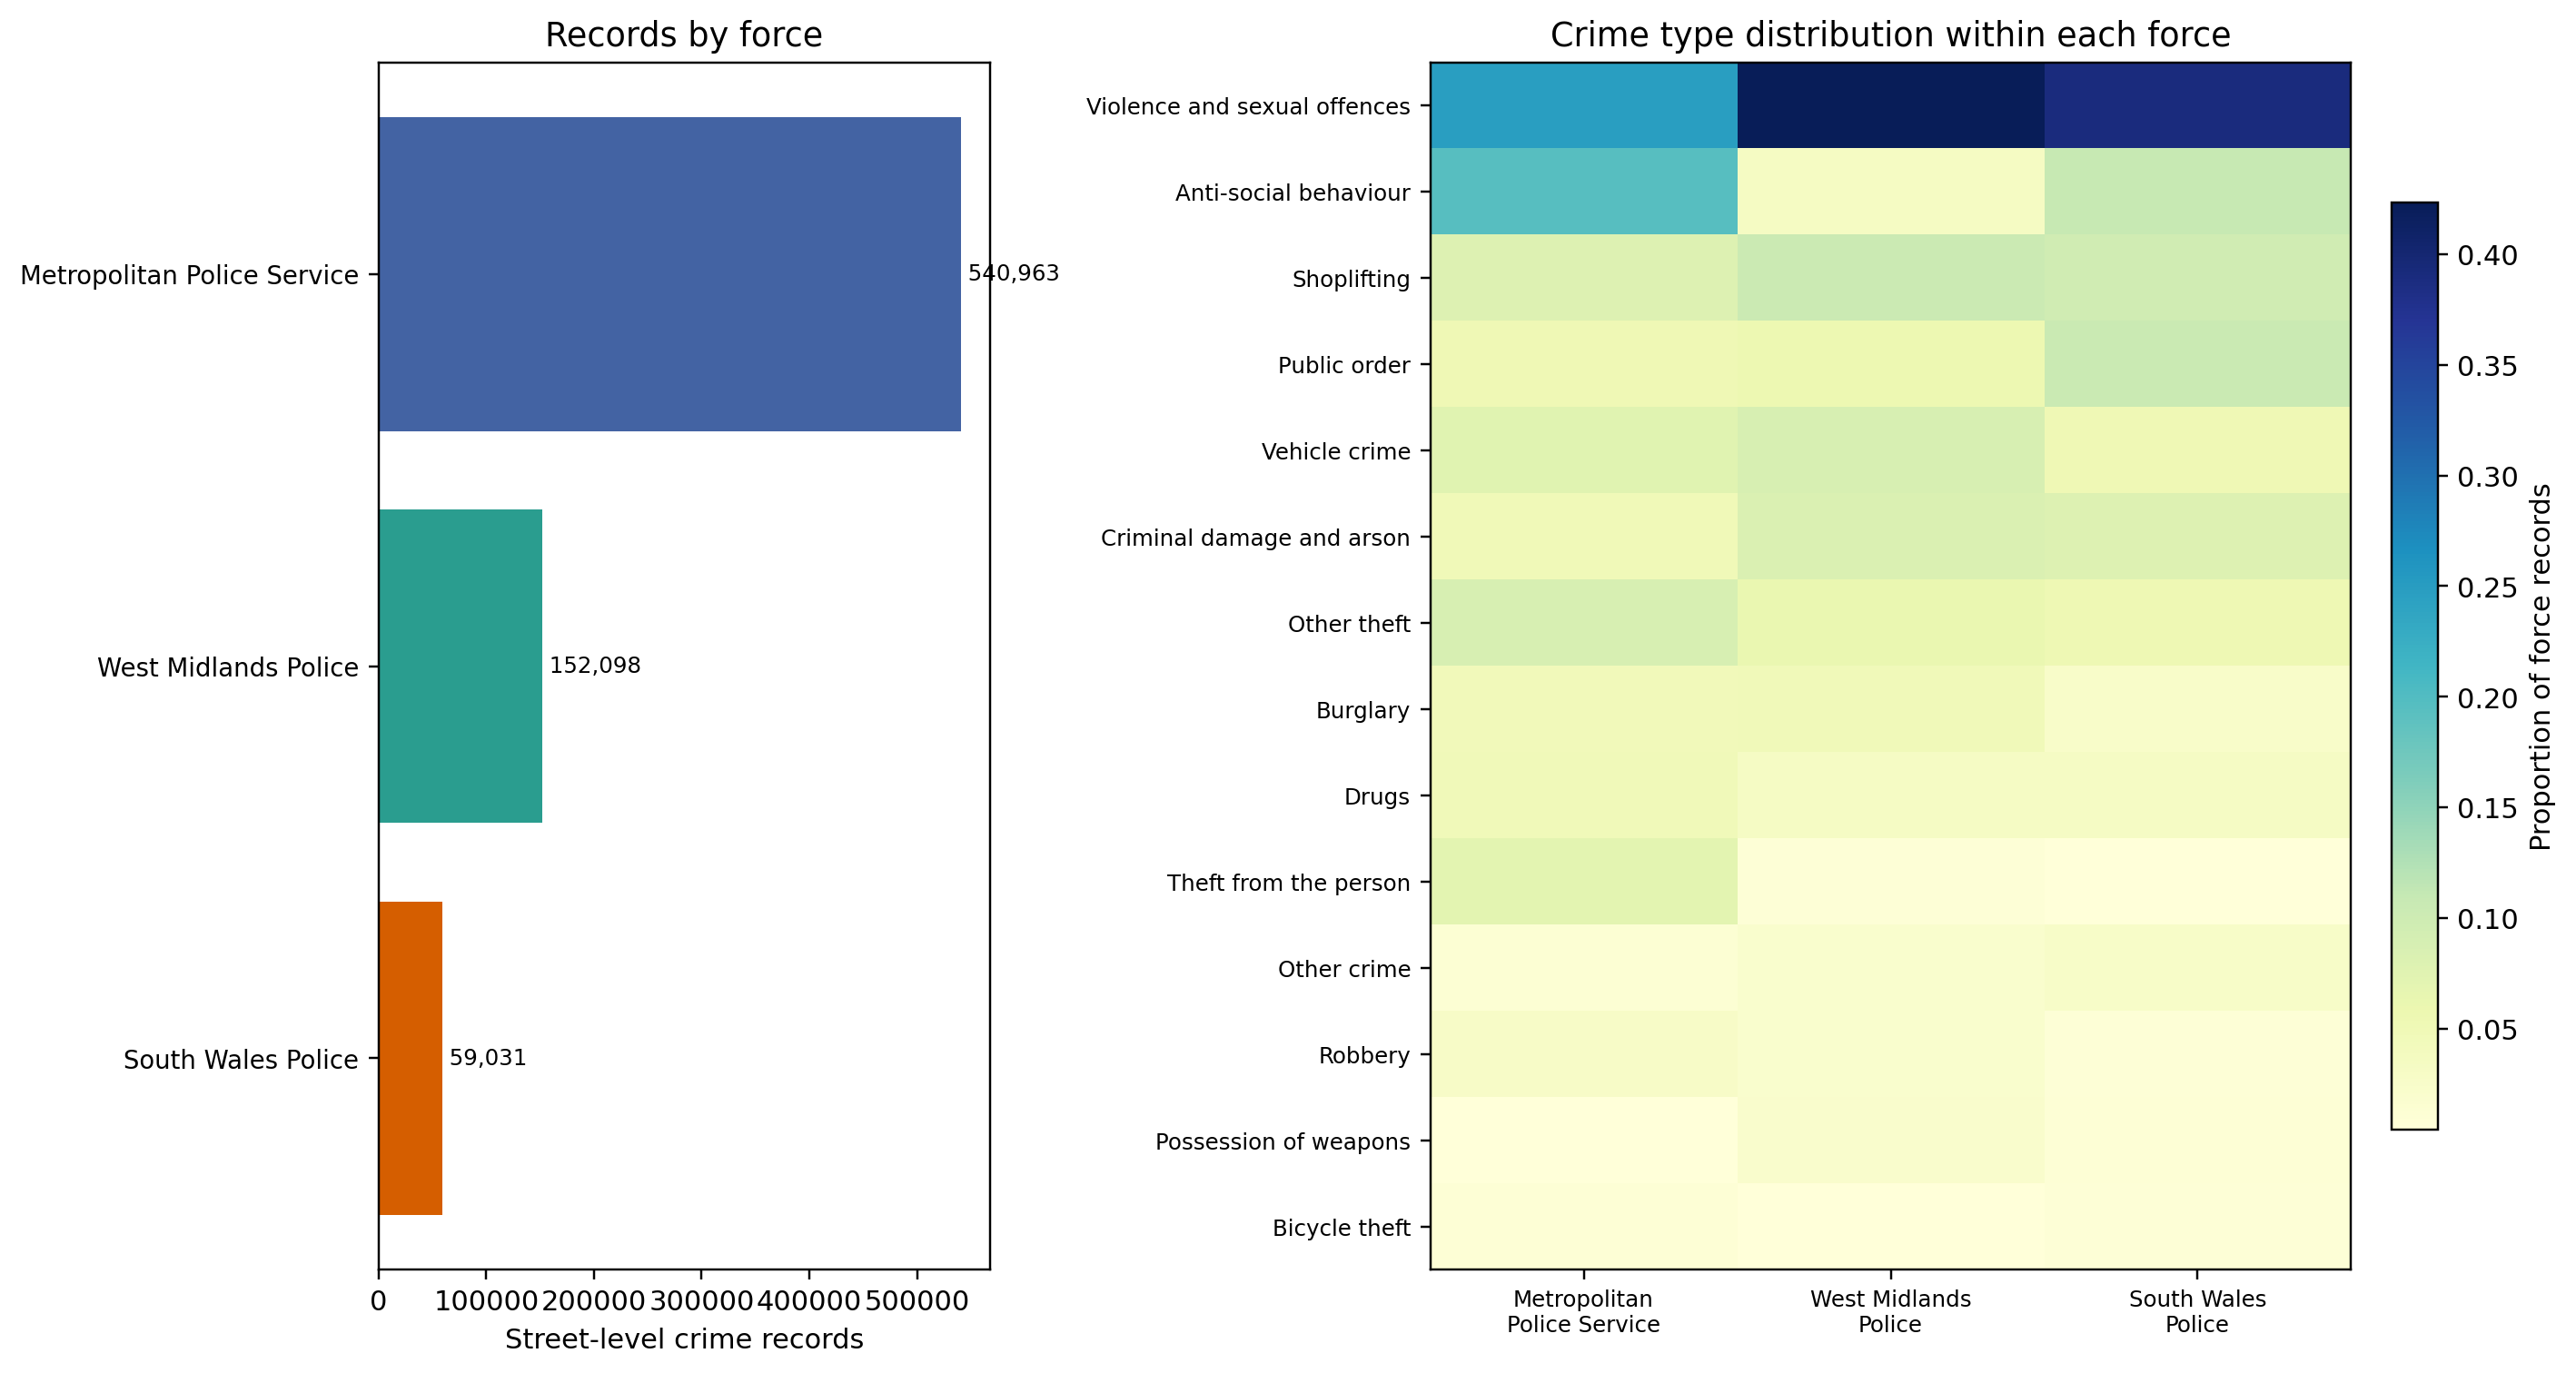
\includegraphics[width=\columnwidth]{figures/fig1_data_overview.png}
\caption{Record volume and crime-type composition across the three
  forces. Metropolitan Police Service has more than nine times the records of
  South Wales; all cross-force comparisons use brokerage scores and
  proportions rather than raw counts.}
\label{fig:data}
\end{figure}

\begin{figure*}[!t]
\centering
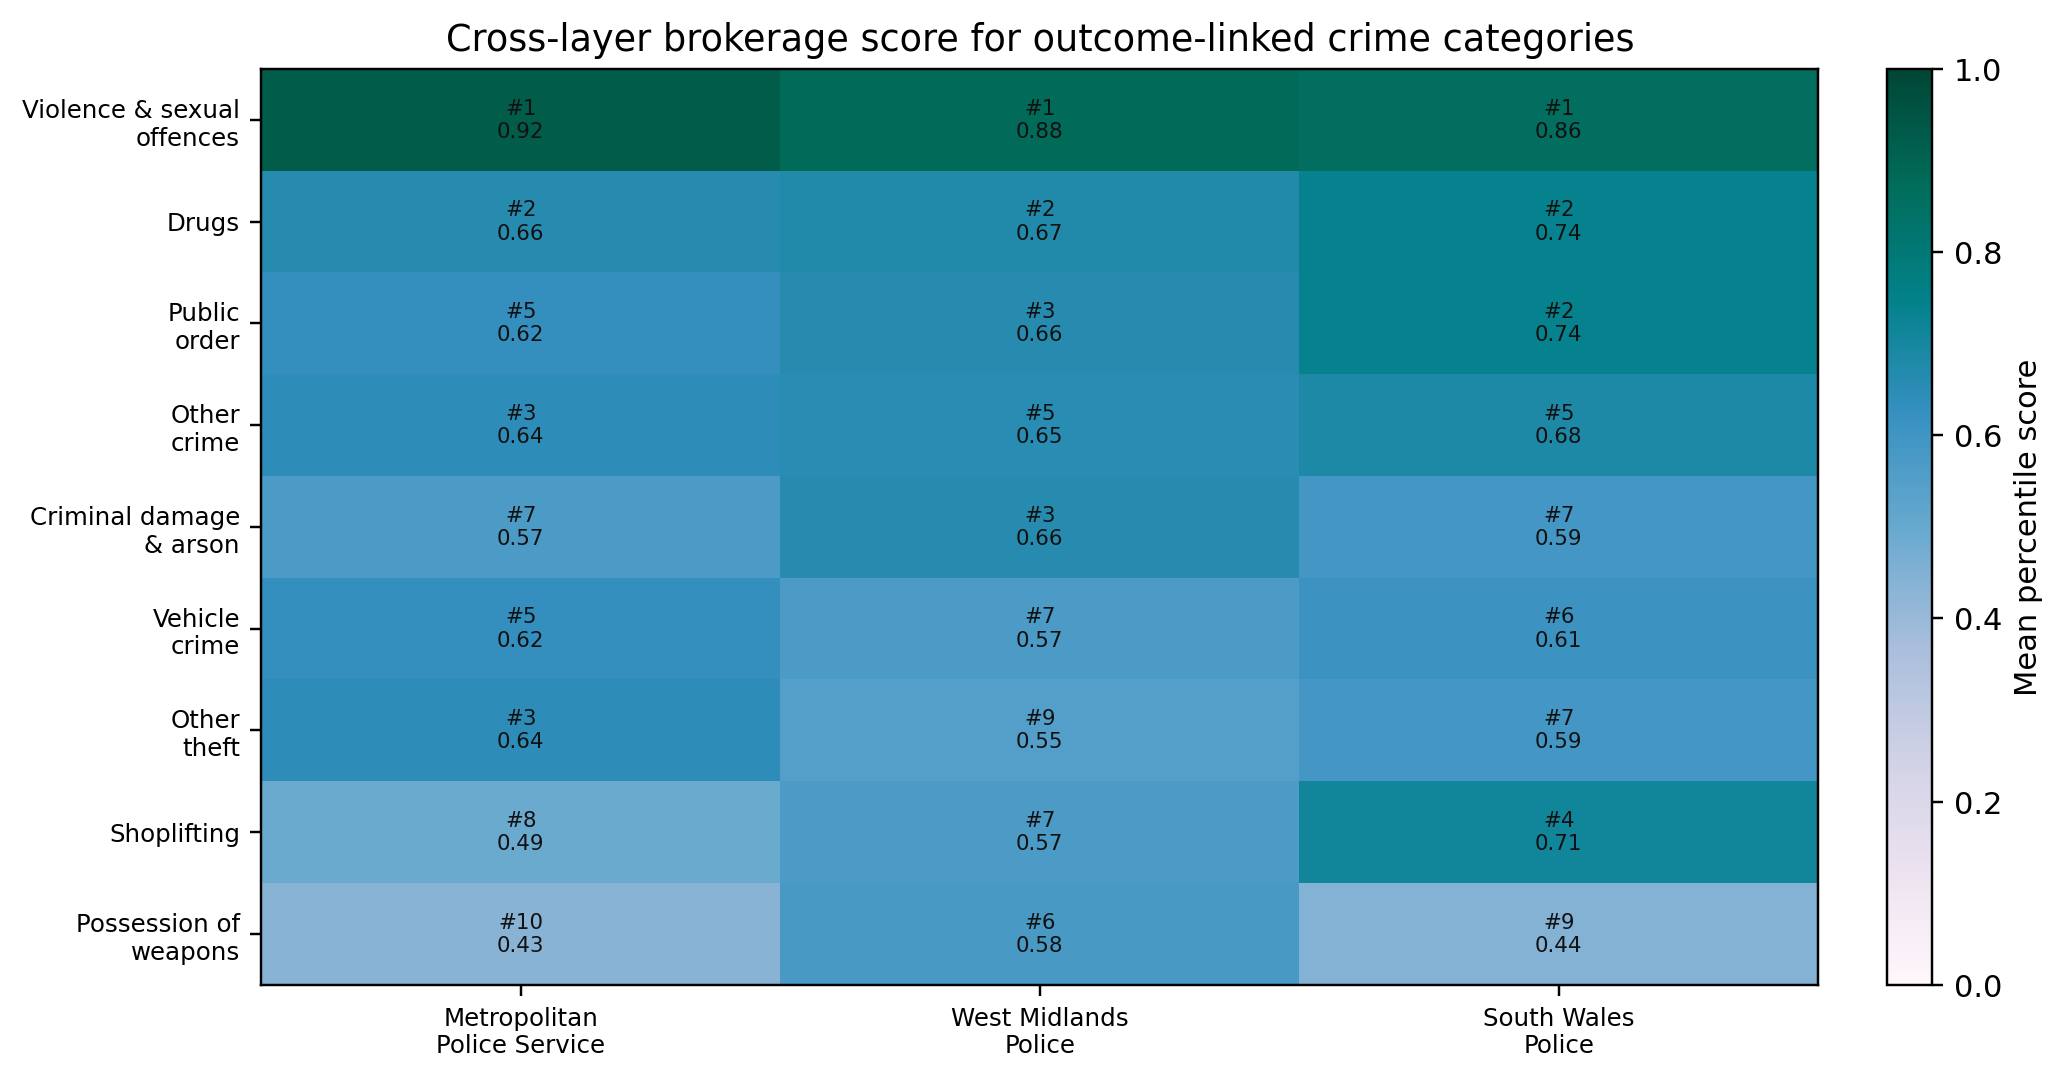
\includegraphics[width=0.72\textwidth]{figures/fig2_brokerage_comparison.png}
\caption{Cross-layer brokerage scores for outcome-linked crime
  categories in each force. Violence and sexual offences ranks first
  in all three forces; drugs ranks second in all three despite not
  appearing in the Metropolitan top five by raw event volume.
  Anti-social behaviour is excluded because its crime-outcome edge
  weight is zero. (top brokers per force shown; equal scores share a
  rank).}
\label{fig:brokerage}
\end{figure*}

\begin{figure*}[!t]
\centering
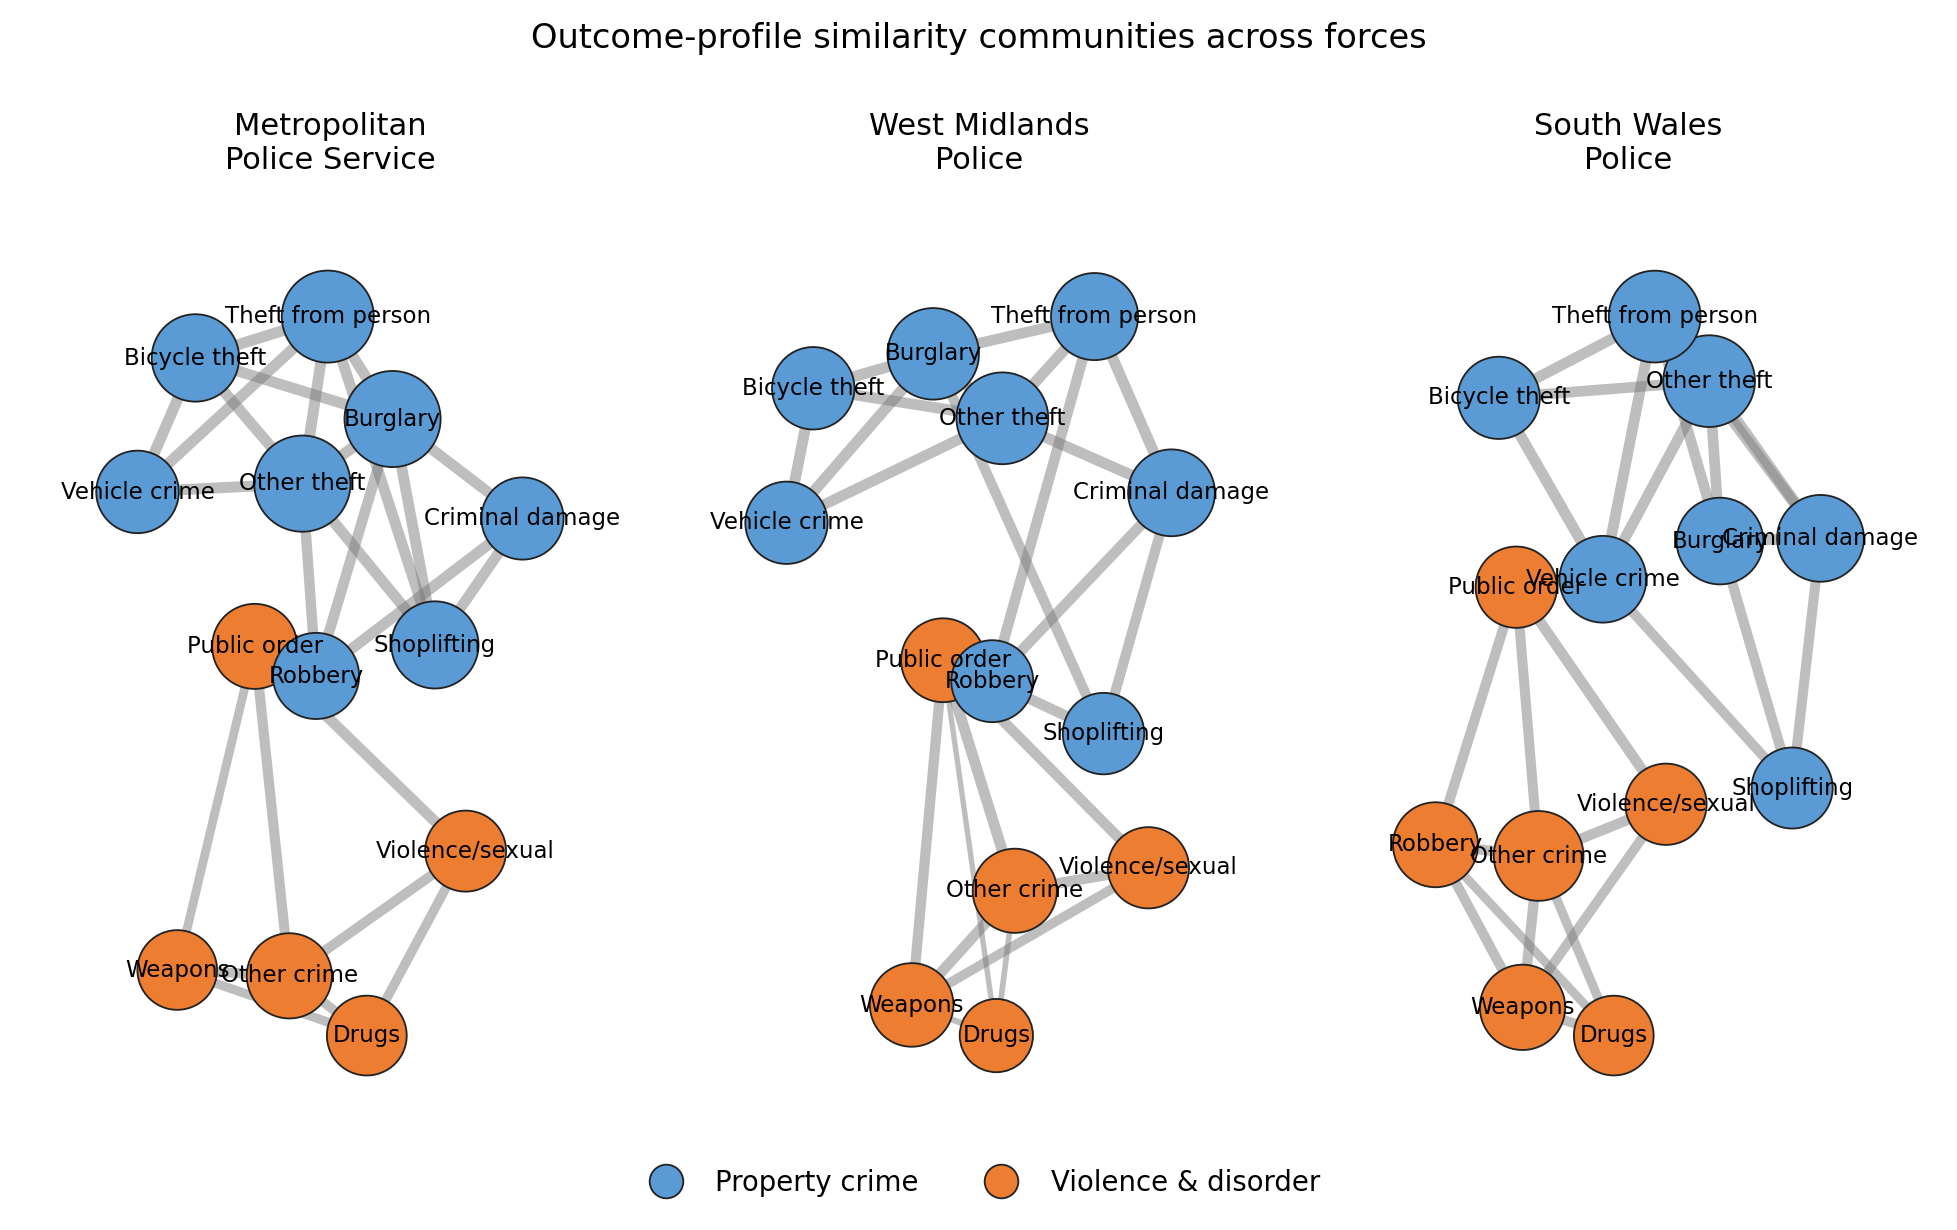
\includegraphics[width=0.68\textwidth]{figures/fig3_similarity_networks.png}
\caption{Outcome-profile similarity networks per force (top-3
  cosine-similarity edges per node). Node colour shows the
  greedy-modularity community relabelled by crime-type membership as
  Property crime or Violence \& disorder, giving consistent colours
  across panels. After semantic relabelling of raw modularity
  communities, the panels show a broadly similar property /
  violence-disorder split;
  robbery shifts between them.}
\label{fig:similarity}
\end{figure*}

Figure~\ref{fig:data} shows the data overview.
Force sizes differ substantially (Table~\ref{tab:data}), so all
subsequent comparisons use brokerage structure and within-force
proportions rather than raw counts.

Figure~\ref{fig:brokerage} shows the brokerage rankings.
Violence and sexual offences ranks first in all three forces (0.92
Metropolitan, 0.88 West Midlands, 0.86 South Wales) with betweenness
concentrated at 0.87, 0.99 and 0.99 respectively.
This concentration is consistent with a hub-like position in the
combined crime network, though this project does not formally test a
scale-free fit.
Drugs ranks second in all three (0.66, 0.67, 0.74).
A raw crime-frequency table for Metropolitan Police Service would not identify
drugs strongly, because several categories have higher event counts.
The composite ranks it second by combining geographic spread, outcome
diversity and path position, properties a frequency table cannot
capture at once, showing what the multilayer framing adds beyond raw
counts.
Second-tier patterns diverge after drugs.
Other crime and other theft lead in Metropolitan, criminal damage and
public order in West Midlands, public order in South Wales.
These differences reflect measured variation in spread and outcome connectivity within the available recorded data.

As a descriptive consistency check, Spearman correlation between brokerage
score and raw area-crime volume was moderate in Metropolitan
($\rho{=}0.57$) and West Midlands ($\rho{=}0.58$) and stronger in
South Wales ($\rho{=}0.85$).
The higher South Wales value may reflect smaller forces: with fewer
LSOAs and less varied structure, spread and volume are harder to
separate, so brokerage converges toward frequency.
Cross-force brokerage correlations were high: 0.85 between Metropolitan
and South Wales, 0.78 between Metropolitan and West Midlands and 0.88
between South Wales and West Midlands, so broker role ordering is
largely consistent across forces despite regional and scale
differences.
PageRank rankings on the combined graph agree closely with betweenness
rankings (Spearman $\rho{=}0.85$ Metropolitan, 0.92 West Midlands, 0.89
South Wales), so the broker ordering does not
depend on the betweenness definition alone.

Figure~\ref{fig:similarity} shows the similarity networks.
After relabelling raw modularity communities by crime-type membership,
all three networks show a property-crime / violence-disorder split;
West Midlands produces three raw modularity communities, which are
collapsed into the broader semantic labels.
The property-crime community groups burglary, vehicle crime, bicycle
theft, other theft, shoplifting and theft from the person, all sharing
outcome profiles dominated by \textit{investigation complete; no
suspect identified} and \textit{unable to prosecute suspect}.
The violence-disorder community groups violence and sexual offences,
drugs, public order, possession of weapons and other crime, with more
distributed outcome profiles.
Robbery shifts from the property community (Metropolitan, West
Midlands) to the violence community (South Wales); the partition is
otherwise broadly similar.
Both the composite score and the similarity communities place drugs
in the diverse-outcome group, matching its elevated entropy.

\paragraph*{Limitations}
Betweenness is approximated ($k{=}250$, fixed seed) on the two larger
graphs and, using inverse-weight distances, remains partly
volume-sensitive.
Area spread counts LSOA presence rather than population-adjusted risk,
which may overstate reach in densely populated areas; LSOAs are
approximate statistical areas, not exact locations.
The six-month window captures one period only, so seasonal patterns
are not visible.
All data is police-recorded crime; no causal claims about crime,
outcomes, or police performance are made.

\vspace{-4pt}
\section{Conclusion}
\vspace{-2pt}

Violence and sexual offences is the dominant cross-layer broker in all
three forces; drugs is a consistent second-tier broker not visible
from raw event-count rankings alone. Broker ordering is broadly
consistent across forces (Spearman 0.78 to 0.88); the same-graph
PageRank comparison gives a similar ordering, suggesting the result is
not purely a betweenness-ranking artefact and the cosine-similarity
community structure aligns with the composite ranking. The consistency
suggests these structural roles may be partly crime-type related,
although differences in recording practices and missing outcome fields
cannot be ruled out.

\clearpage
\onecolumn
\appendix
\subsection*{Centrality-metric comparison}
\vspace{-4pt}

\begin{figure}[H]
\centering
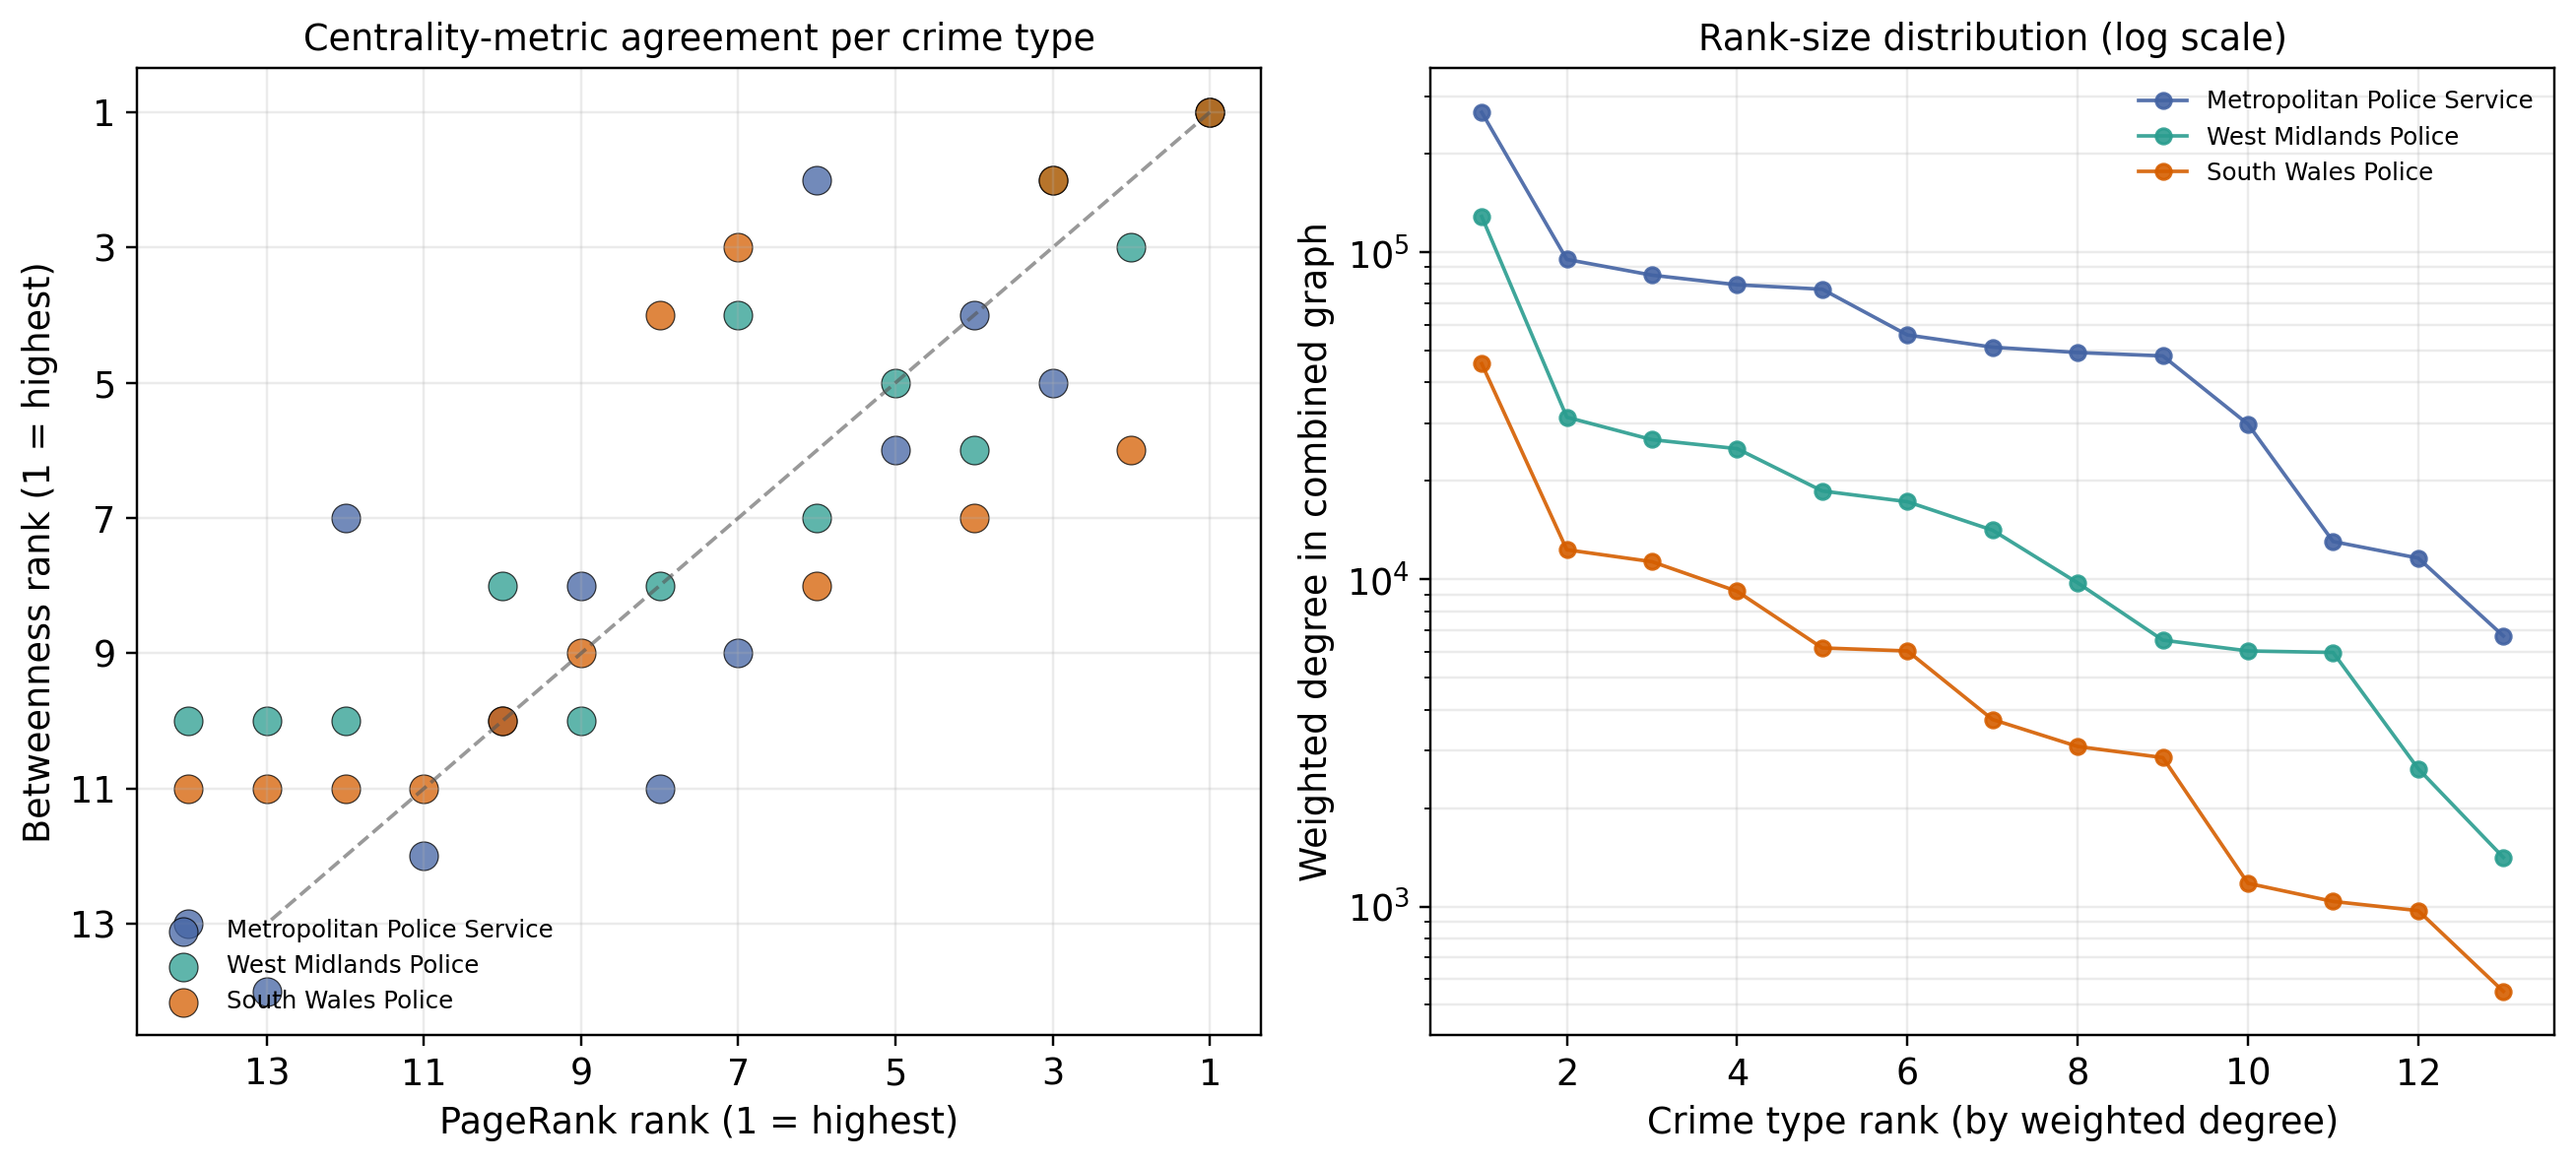
\includegraphics[width=0.92\textwidth]{figures/fig4_centrality_comparison.png}
\vspace{-8pt}
\caption{Centrality-metric comparison. Left: PageRank rank vs
  betweenness rank per crime type; points near the dashed diagonal
  indicate the two metrics agree. Right: weighted-degree rank-size
  distribution of crime nodes in the combined graph, log-scaled;
  the steep drop from rank 1 is consistent with a highly concentrated
  weighted-degree distribution.}
\label{fig:centrality}
\end{figure}
\vspace{-8pt}

Figure~\ref{fig:centrality} shows two supporting views of the combined
crime network. Left: PageRank rank against betweenness rank per
brokerage-eligible category; points near the diagonal indicate
agreement and violence and sexual offences sits at rank 1 for both
metrics in all three forces. Right: rank-size distribution of weighted
node degree on a log scale; the steep drop from the top-ranked
category is consistent with a highly concentrated weighted-degree
distribution without formally testing a scale-free fit.

\vspace{-6pt}
\subsection*{Future work}

Longer time windows would allow temporal-stability tests using
leave-one-month-out resampling of the brokerage hierarchy.
Area spread should be normalised by LSOA population to remove the
implicit weighting toward densely populated areas.
Additional forces would test whether the property-crime /
violence-disorder community structure generalises beyond England and
Wales and inclusion of stop-and-search data, once outcome
comparability is resolved, would extend the crime-outcome layer.

\bibliographystyle{IEEEtran}
\bibliography{references}

\end{document}
